%input macros (i.e. write your own macros file called MacroFile1.tex)
%\newcommand{\PdfPsText}[2]{
  \ifpdf
     #1
  \else
     #2
  \fi
}

\newcommand{\IncludeGraphicsH}[3]{
  \PdfPsText{\includegraphics[height=#2]{#1}}{\includegraphics[bb = #3, height=#2]{#1}}
}

\newcommand{\IncludeGraphicsW}[3]{
  \PdfPsText{\includegraphics[width=#2]{#1}}{\includegraphics[bb = #3, width=#2]{#1}}
}

\newcommand{\InsertFig}[3]{
  \begin{figure}[!htbp]
    \begin{center}
      \leavevmode
      #1
      \caption{#2}
      \label{#3}
    \end{center}
  \end{figure}
}


%%% Local Variables: 
%%% mode: latex
%%% TeX-master: "~/Documents/LaTeX/CUEDThesisPSnPDF/thesis"
%%% End: 


 \documentclass[oneside,12pt]{Classes/CUEDthesisPSnPDF}


\ifpdf
    \pdfinfo { /Title  (CUED PhD and MPhil Thesis Classes)
               /Creator (TeX)
               /Producer (pdfTeX)
               /Author (Harish Bhanderi harish.bhanderi@cantab.net)
               /CreationDate (D:20030101000000)  %format D:YYYYMMDDhhmmss
               /ModDate (D:20030815213532)
               /Subject (Writing a PhD thesis in LaTeX)
               /Keywords (PhD, Thesis)}
    \pdfcatalog { /PageMode (/UseOutlines)
                  /OpenAction (fitbh)  }
\fi

\title{Writing a PhD Thesis\\[1ex]
        in \LaTeXe}

\ifpdf
  \author{\href{mailto:harish.bhanderi@cantab.net}{Harish Bhanderi}}
  \collegeordept{\href{http://www.eng.cam.ac.uk}{Department of Engineering}}
  \university{\href{http://www.cam.ac.uk}{University of Cambridge}}
% insert below the file name that contains the crest in-place of 'UnivShield'
  \crest{
\includegraphics[width=30mm]{UnivShield}}
\else
  \author{Harish Bhanderi}
  \collegeordept{Department of Engineering}
  \university{University of Cambridge}
% insert below the file name that contains the crest in-place of 'UnivShield'
  \crest{
\includegraphics[bb = 0 0 292 336, width=30mm]{UnivShield}}
\fi
%
% insert below the file name that contains the crest in-place of 'UnivShield'
% \crest{\IncludeGraphicsW{UnivShield}{40mm}{14 14 73 81}}
%
%\renewcommand{\submittedtext}{change the default text here if needed}
\degree{Doctor of Philosophy}
\degreedate{Yet to be decided}

% turn of those nasty overfull and underfull hboxes
\hbadness=10000
\hfuzz=50pt

% Put all the style files you want in the directory StyleFiles and usepackage like this:
\usepackage{StyleFiles/watermark}
\usepackage[version=3]{mhchem}

% - use EPS with pdfLaTeX, essential for chemscheme ----
%\usepackage[runs=2]{auto-pst-pdf}
\usepackage[journal=rsc]{chemstyle}
\usepackage{chemmacros}

\usepackage{siunitx}

\usepackage[T1]{fontenc}
\usepackage{lmodern}
\usepackage{geometry} % Easy page layou

% - optional command that make compound names easier to see ----
\renewcommand*{\schemerefformat}{%
  \color{magenta}\textit
}%

\doublespacing

\begin{document}

%\language{english}

% A page with the abstract on including title and author etc may be
% required to be handed in separately. If this is not so, then comment
% the below 3 lines (between '\begin{abstractseparte}' and
% 'end{abstractseparate}'), normally like a declaration ... needs some more
% work, mind as environment abstracts creates a new page!
% \begin{abstractseparate}
%   
% Thesis Abstract -----------------------------------------------------


%\begin{abstractslong}    %uncommenting this line, gives a different abstract heading
\begin{abstracts}        %this creates the heading for the abstract page

This is where you write your abstract ...


\end{abstracts}
%\end{abstractlongs}


% ----------------------------------------------------------------------


%%% Local Variables: 
%%% mode: latex
%%% TeX-master: "../thesis"
%%% End: 

% \end{abstractseparate}




% Using the watermark package which is in StyleFiles/
% and to remove DRAFT COPY ONLY appearing on the top of all pages comment out below line
%\watermark{DRAFT COPY ONLY}


\maketitle

%set the number of sectioning levels that get number and appear in the contents
\setcounter{secnumdepth}{3}
\setcounter{tocdepth}{3}

\frontmatter % book mode onlyd
\pagenumbering{roman}
% Thesis Acknowledgements ------------------------------------------------


%\begin{acknowledgementslong} %uncommenting this line, gives a different acknowledgements heading
\begin{acknowledgements}      %this creates the heading for the acknowlegments


And I would like to acknowledge ...


\end{acknowledgements}
%\end{acknowledgmentslong}

% ------------------------------------------------------------------------

%%% Local Variables: 
%%% mode: latex
%%% TeX-master: "../thesis"
%%% End: 


% Thesis Abstract -----------------------------------------------------


%\begin{abstractslong}    %uncommenting this line, gives a different abstract heading
\begin{abstracts}        %this creates the heading for the abstract page

This is where you write your abstract ...


\end{abstracts}
%\end{abstractlongs}


% ----------------------------------------------------------------------


%%% Local Variables: 
%%% mode: latex
%%% TeX-master: "../thesis"
%%% End: 


\tableofcontents
\listoffigures
\listofschemes
\printnomenclature  %% Print the nomenclature
\addcontentsline{toc}{chapter}{Nomenclature}

\mainmatter % book mode only
%%% Thesis Introduction --------------------------------------------------
\chapter{Introduction}
\ifpdf
    \graphicspath{{Introduction/IntroductionFigs/PNG/}{Introduction/IntroductionFigs/PDF/}{Introduction/IntroductionFigs/}}
\else
    \graphicspath{{Introduction/IntroductionFigs/EPS/}{Introduction/IntroductionFigs/}}
\fi

And this is how I would like to introduce my piece of work ...


blah blah blah blah blah blah blah blah blah blah blah blah blah blah blah blah blah blah blah blah blah blah blah blah blah blah blah blah blah blah blah blah blah blah blah blah blah blah blah blah blah blah blah blah blah blah blah blah blah blah blah blah blah blah blah blah blah blah blah blah blah blah blah blah blah blah blah blah blah blah blah blah blah blah blah blah blah blah blah blah blah blah blah blah blah blah blah blah blah blah blah blah blah blah blah blah blah blah blah blah blah blah blah blah blah blah blah blah blah blah blah blah blah blah blah blah blah blah blah blah blah blah blah blah blah blah blah blah blah blah blah blah blah blah blah blah blah blah blah blah blah blah blah blah blah blah blah blah blah blah blah blah blah blah blah blah blah blah blah blah blah blah blah blah blah blah blah blah blah blah blah blah blah blah blah blah blah blah blah blah blah blah blah blah blah blah blah blah blah blah blah blah blah blah blah blah blah blah blah blah blah blah blah blah blah blah blah blah blah blah blah blah blah blah blah blah blah blah blah blah blah blah blah blah blah blah blah blah blah blah blah blah blah blah blah blah blah blah blah blah blah blah blah blah blah blah blah blah blah blah blah blah blah blah blah blah blah blah blah blah blah blah blah blah blah blah blah blah blah blah blah blah blah blah blah blah blah blah blah blah blah blah blah blah blah blah blah blah blah blah blah blah blah blah blah blah blah blah blah blah blah blah blah blah blah blah blah blah blah blah blah blah blah blah blah blah blah blah blah blah blah blah blah blah blah blah blah blah blah blah blah blah blah blah blah blah blah blah blah blah blah blah blah blah blah blah blah blah blah blah blah blah blah blah blah blah blah blah blah blah blah blah blah blah blah blah blah blah blah blah blah blah blah blah blah blah blah blah blah blah blah blah blah blah blah blah blah blah blah blah blah blah blah blah blah blah blah blah blah blah blah blah blah blah blah blah blah blah blah blah blah blah blah blah blah blah blah blah blah blah blah blah blah blah blah blah blah blah blah blah blah blah blah blah blah blah blah blah blah blah blah blah blah blah blah blah blah blah blah blah blah blah blah blah blah blah blah blah blah blah blah blah blah blah blah blah blah blah blah blah blah blah blah blah blah blah blah blah blah blah blah blah blah blah blah blah blah blah blah blah blah blah blah blah blah blah blah blah blah blah blah blah blah blah blah blah blah blah blah blah blah blah blah blah blah blah blah blah blah blah blah blah blah blah blah blah blah blah blah blah blah blah blah blah blah blah blah blah blah blah blah blah blah blah blah blah blah blah blah blah blah blah blah blah blah blah blah blah blah blah blah blah blah blah blah blah blah blah blah blah blah blah blah blah blah blah blah blah blah blah blah blah blah blah blah blah blah blah blah blah blah blah blah blah blah blah blah blah blah blah blah blah blah blah blah blah blah blah blah blah blah blah blah blah blah blah blah blah blah blah blah blah blah blah blah blah blah blah blah blah blah blah blah blah blah blah blah blah blah blah blah blah blah blah blah blah blah blah blah blah blah blah blah blah blah blah blah blah blah blah blah blah blah blah blah blah blah blah blah blah blah blah blah blah blah blah blah blah blah blah blah blah blah blah blah blah blah blah blah blah blah blah blah blah blah blah blah blah blah blah blah blah blah blah blah blah blah blah blah blah blah blah blah blah blah blah blah blah blah blah blah blah blah blah blah blah blah blah blah blah blah blah blah blah blah blah blah blah blah blah blah blah blah blah blah blah blah blah blah blah blah blah blah blah blah blah blah blah blah blah blah blah blah blah blah blah blah blah blah blah blah blah blah blah blah blah blah blah blah blah blah blah blah blah blah blah blah blah blah blah blah blah blah blah blah blah blah blah blah blah blah blah blah blah blah blah blah blah blah blah blah blah blah blah blah blah blah blah blah blah blah blah blah blah blah blah blah blah blah blah blah blah blah blah blah blah blah blah blah blah blah blah blah blah blah blah blah blah blah blah blah blah blah blah blah blah blah blah blah blah blah blah blah

%%% ----------------------------------------------------------------------


%%% Local Variables: 
%%% mode: latex
%%% TeX-master: "../thesis"
%%% End: 

% \pagebreak[4]
% \hspace*{1cm}
% \pagebreak[4]
% \hspace*{1cm}
% \pagebreak[4]

\chapter{Results and Discussion}
\ifpdf
    \graphicspath{{Results/ResultsFigs/PNG/}{Results/ResultsFigs/PDF/}{Results/ResultsFigs/}}
\else
    \graphicspath{{Results/ResultsFigs/EPS/}{Results/ResultsFigs/}}
\fi

\section{Synthesis of S-protected 2-mercapto-2-phenylacetaldehyde ligation auxillaries}


The expeiments conducted and results are set out and described. Results should be discussed and set in context with the recent literature so that their significance is evident. A clear story should be developed so that the reader is lead through the project, understanding why experiments were performed and the  relevance of the results at each stage. The R\&D section should lead on from the introduction, and into the conclusion, building on ideas from the introduction and clearly highlighting key results for the conclusion.

And now I begin my first chapter here ...

Here is an equation\footnote{the notation is explained in the nomenclature section :-)}:
\begin{eqnarray}
CIF: \hspace*{5mm}F_0^j(a) &=& \frac{1}{2\pi \iota} \oint_{\gamma} \frac{F_0^j(z)}{z - a} dz
\end{eqnarray}
\nomenclature[zcif]{$CIF$}{Cauchy's Integral Formula}                                % first letter Z is for Acronyms
\nomenclature[aF]{$F$}{complex function}                                                   % first letter A is for Roman symbols
\nomenclature[gp]{$\pi$}{ $\simeq 3.14\ldots$}                                             % first letter G is for Greek Symbols
\nomenclature[gi]{$\iota$}{unit imaginary number $\sqrt{-1}$}                      % first letter G is for Greek Symbols
\nomenclature[gg]{$\gamma$}{a simply closed curve on a complex plane}  % first letter G is for Greek Symbols
\nomenclature[xi]{$\oint_\gamma$}{integration around a curve $\gamma$} % first letter X is for Other Symbols
\nomenclature[rj]{$j$}{superscript index}                                                       % first letter R is for superscripts
\nomenclature[s0]{$0$}{subscript index}                                                        % first letter S is for subscripts

\subsection{Second Paragraph}
and here I write more ...\cite{texbook}

\subsection{sub first paragraph}
... and some more ...

Now I would like to cite the following: \cite{latex} and \cite{texbook}
and \cite{Rud73}.

I would also like to include a picture ...

\begin{figure}[!htbp]
  \begin{center}
    \leavevmode
    \ifpdf
      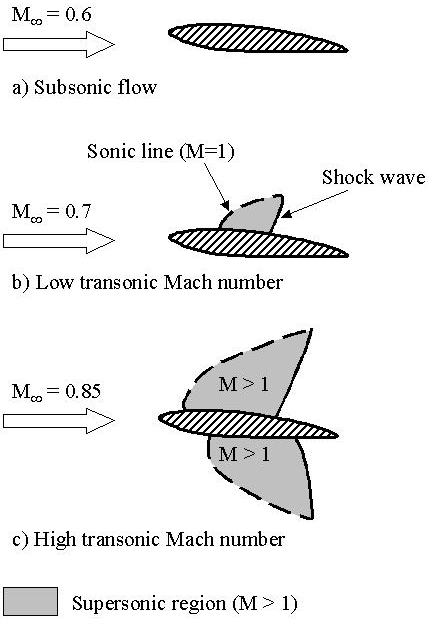
\includegraphics[height=6in]{aflow}
    \else
      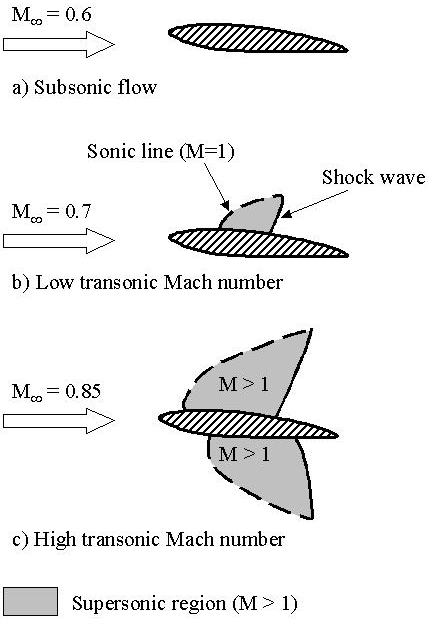
\includegraphics[bb = 92 86 545 742, height=6in]{aflow}
    \fi
    \caption{Airfoil Picture}
    \label{FigAir}
  \end{center}
\end{figure}

% above code has been macro-fied in Classes/MacroFile.tex file
%\InsertFig{\IncludeGraphicsH{aflow}{6in}{92 86 545 742}}{Airfoil Picture}{FigAir}

So as we have now labelled it we can reference it, like so (\ref{FigAir}) and it
is on Page \pageref{FigAir}. And as we can see, it is a very nice picture and we
can talk about it all we want and when we are tired we can move on to the next
chapter ...

I would also like to add an extra bookmark in acroread like so ...
\ifpdf
  \pdfbookmark[2]{bookmark text is here}{And this is what I want bookmarked}
\fi
% ------------------------------------------------------------------------


%%% Local Variables:
%%% mode: latex
%%% TeX-master: "../thesis"
%%% End:

\def\baselinestretch{1}
\chapter{My Conclusions ...}
\ifpdf
    \graphicspath{{Conclusions/ConclusionsFigs/PNG/}{Conclusions/ConclusionsFigs/PDF/}{Conclusions/ConclusionsFigs/}}
\else
    \graphicspath{{Conclusions/ConclusionsFigs/EPS/}{Conclusions/ConclusionsFigs/}}
\fi

\def\baselinestretch{1.66}

Here I put all my conclusions ...

%%% ----------------------------------------------------------------------

% ------------------------------------------------------------------------

%%% Local Variables:
%%% mode: latex
%%% TeX-master: "../thesis"
%%% End:

\chapter{Experimental Methods}
\ifpdf
    \graphicspath{{Experimental/ExperimentalFigs/PNG/}{Experimental/ExperimentalFigs/PDF/}{Experimental/ExperimentalFigs/}}
\else
    \graphicspath{{Experimental/ExperimentalFigs/EPS/}{Experimental/ExperimentalFigs/}}
\fi

%%%%%%%%%%%%%%%%%%%%%%%%%%%%%%%%%%%%%%%%%%%%%%%%%%%%%%%%%%%%

\section{2-bromo-2-(4-bromophenyl)acetic acid}
\begin{scheme}[ht]
    \schemeref[TMP1]{cmpd:4BrPAA}
    \schemeref[TMP2]{cmpd:dibromoPAA}
    \includegraphics{4-BrPAA-bromination.eps}
    \caption{Benzylic Bromination of \compound{cmpd:4-BrPAA}.\label{sch:BenzylBromination}}
\end{scheme}

\begin{experimental}[delta=(ppm),pos-number=sub,use-equal]
  \sisetup{separate-uncertainty,per-mode=symbol,detect-all,range-phrase=--}

A mixture of carboxylic acid \compound{cmpd:4BrPAA} (\SI{10.6}{\gram}, \SI{46.5}{\milli\mol}) and \ce{N-bromosuccinimide} (\SI{9.932}{\gram}, \SI{55.8}{\milli\mol}) were suspended in \ce{CCl4} (\SI{250}{\milli\L}) and the mixture was irradiated under refluxed with a \SI{240}{\watt} tungsten lamp.

An NMR of the crude mixture after three hours indicated incomplete conversion of the starting material. An additional 0.5 eq of NBS was addded and the reaction was again irradiated under reflux for a furthur 3 hours. The mixture was cooled, filtered, and the solvent along with elemental bromine were removed \invacuo. The residual orange solid was purified by flash column chromatography (2:1 Cyclohexane:Ethyl Acetate + \SI{1}{\percent} formic acid). Formic acid was coevaporated from the product with ethyl acetate to yield an off-white crystalline solid (\compound{cmpd:dibromoPAA}, \SI{9.733}{\gram}, \SI{71}{\percent}).

\NMR(500)[CDCl3] \val{5.31} (s, \#{1}, \pos{5}), \val{7.42--7.45} (m, \#{2}, \pos{11}), \val{7.50--7.53} (m, \#{2}, \pos{11}.
%
\NMR{13,C}(150)[CDCl3] \val{44.72} ($+$, \#{1}, \pos{1}), \val{23.4} ($+$,
\#{8}, \pos{5}), \val{126.0} ($+$, \#{4}, \pos{9}), \val{128.2} ($+$, \#{8},
\pos{3}), \val{130.8} ($+$, \#{2}, \pos{12}), \val{133.6} ($+$, \#{2},
\pos{11}), \val{137.0} ($+$, \#{4}, \pos{8}), \val{138.6} (q, \#{4},
\pos{2}), \val{140.6} (q, \#{2}, \pos{10}), \val{140.8} (q, \#{8}, \pos{4}),
\val{141.8} (q, \#{4}, \pos{6}), \val{145.6} (q, \#{2}, \pos{7})
%
  % \data{MS}[DCP, EI, \SI{60}{\electronvolt}] \val{703} (2, \ch{M+}), \val{582}
  % (1), \val{462} (1), \val{249} (13), \val{120} (41), \val{105} (100).
  % %
  % \data{MS}[\ch{MeOH + H2O + KI}, ESI, \SI{10}{\electronvolt}] \val{720} (100,
  % \ch{M+ + OH-}), \val{368} (\ch{M+ + 2 OH-}).
  % %
  % \data{IR}[KBr] \val{3443} (w), \val{3061} (w), \val{2957} (m), \val{2918}
  % (m), \val{2856} (w), \val{2729} (w), \val{1725} (w), \val{1606} (s),
  % \val{1592} (s), \val{1545} (w), \val{1446} (m), \val{1421} (m), \val{1402}
  % (m), \val{1357} (w), \val{1278} (w), \val{1238} (s), \val{1214} (s),
  % \val{1172} (s), \val{1154} (m), \val{1101} (w), \val{1030} (w), \val{979}
  % (m), \val{874} (m), \val{846} (s), \val{818} (w), \val{798} (m), \val{744}
  % (w), \val{724} (m), \val{663} (w), \val{586} (w), \val{562} (w), \val{515}
  % (w).
  %
\end{experimental}

%%%%%%%%%%%%%%%%%%%%%%%%%%%%%%%%%%%%%%%%%%%%%%%%%%%%%%%%%%%%

\section{2-bromo-2-(4-bromophenyl)-N-methoxy-N-methylacetamide}
To a stirred solution of \compound{cmpd:dibromoPAA} (\SI{4.409}{\gram}, \SI{15}{\milli\mol}) in dry DCM (\SI{120}{\milli\litre}) under argon at \SI{0}{\celsius} was added N,O-dimethylhydroxylamine hydrochloride (\SI{1.463}{\gram}, \SI{15}{\milli\mol}) followed by 1-(3-Dimethylaminopropyl)-3-ethylcarbodiimide hydrochloride (\SI{3.019}{\gram}, \SI{15.75}{\milli\mol}) in portions over \SI{15}{\minute}. Triethylamine (\SI{3.14}{\milli\litre}, \SI{22.5}{\milli\mol}) was then added and the mixture was allowed to rise to room temperature after stirring at \SI{0}{\celsius} for a further \SI{15}{\minute}.

After \SI{1}{\hour} the reaction mixture was washed with aq. \ce{HCl} (\SI{1}{\Molar}, 3x\SI{50}{\milli\litre}), sat. \ce{NaHCO3} (3x\SI{50}{\milli\litre}), brine (1x\SI{50}{\milli\litre}) and dried over \ce{MgSO4}. The solvent was removed \invacuo to yield \compound{dibromoamide} as a clear yellow oil which was not further purified.

%%%%%%%%%%%%%%%%%%%%%%%%%%%%%%%%%%%%%%%%%%%%%%%%%%%%%%%%%%%%

\section{S-(1-(4-bromophenyl)-2-(methoxy(methyl)amino)-2-oxoethyl) O-ethyl carbonodithioate}

A solution of \compound{dibromoamide} (\SI{4.586}{\gram}, \SI{13.6}{\milli\mol}) and potassium ethyl xanthate in acetone {\SI{100}{\milli\litre}} was  stirred at room temperature for \SI{3}{\hour} at which point TLC indicate complete consumption of the starting material. The solvent was remove \invacuo to yield a yellow oil which was taken up in water, extracted with \ce{DCM} (2x\SI{50}{\milli\litre}), the organics dried over \ce{MgSO4} and the solvent remove to yield a yellow oil which formed a crystalline solid on standing overnight. The solid was purified by column chromatography (2:1 cyclohexane:ethyl acetate) to yield \compound{cmpd:bromoxanthateamide} as a perlescent white crystaline solid (\SI{4.3523}{\gram}, \SI{11.5}{\milli\mol}, \SI{84.5}{\percent}) on standing overnight.

%%%%%%%%%%%%%%%%%%%%%%%%%%%%%%%%%%%%%%%%%%%%%%%%%%%%%%%%%%%%

\section{2-(4-bromophenyl)-2-mercapto-N-methoxy-N-methylacetamide}

Piperidine (\SI{1.02}{\milli\litre}, \SI{10.2}{\milli\mol}) was added dropwise to a stirred mixture of \compound{cmpd:bromoxanthateamide} (\SI{3.4714}{\gram}, \SI{9.2}{\milli\mol}) in dry \ce{DCM} which had been deoxygenated by repeated argon/vacuum purges and placed under argon on a ice/water bath. TLC indicated that starting material remained after \SI{1}{\hour} at which point an additional 0.2 eq of \ch{piperidine} was added followed by another 0.4 eq in two portions.

The reaction was stopped with the addition of aq. \ce{HCl} (\SI{1}{\Molar}, \SI{50}{\milli\litre}), the organics were separated, washed with \ce{HCl} (\SI{1}{\Molar}, 2x\SI{50}{\milli\litre}, brine {\SI{50}{\milli\litre}), dried over \ce{MgSO4}, and the solvent removed \invacuo. The residue was purified by flash chromotography (2:1 \ce{cyclohexane}:\ce{ethyl acetate} + \SI{1}{\percent} formic acid) to yield starting material, a mixed fraction and an oil which crystalised as a white solid \compound{cmpd:bromothioamide} on cooling (\SI{1.083}{\gram}, \SI{3.82}{\milli\mol}, \SI{37.4}{\percent}).

%%%%%%%%%%%%%%%%%%%%%%%%%%%%%%%%%%%%%%%%%%%%%%%%%%%%%%%%%%%%

\section{2-(4-bromophenyl)-N-methoxy-N-methyl-2-(4,4'-dimethoxytritylthio)acetamide}

To a stirred solution of \compound{cmpd:bromothioamide} (\SI{1.069}{\gram}, \SI{3.68}{\milli\mol}) in DCM was added \ce{4,4'-dimethoxytrityl chloride} (\SI{1.372}{\gram}, \SI{4.05}{\milli\mol}) followed by triethylamine (\SI{0.56}{\milli\litre}, \SI{4.05}{\milli\mol}). After \SI{1}{\hour} an additional 0.2 eq of \ce{4,4'-DMT.Cl} and triethylamine were added. The reaction was worked up after a further \SI{30}{\minute} by washing the organics with water (2x\SI{70}{\milli\litre}), drying over \ce{MgSO4}, and removing the solvent \invacuo. The crude was purified by flash column chromatography (gradiant from 6:1 to 2:1 \ce{cyclohexane}:\ce{ethyl acetate} + \SI{0.5}{\percent} \ce{dimethylethylamine}) to yield \compound{cmpd:bromoDMTamide} as a fine white crystalline solid (\SI{1.8419}{\gram}, \SI{3.1}{\milli\mol}, \SI{84}{\percent}).

%%%%%%%%%%%%%%%%%%%%%%%%%%%%%%%%%%%%%%%%%%%%%%%%%%%%%%%%%%%%

\section{2-(4-bromophenyl)-2-(4,4'-dimethoxytritylthio)acetaldehyde}

A solution of \ce{LiAlH4} (\SI{3}{\Molar} in \ce{THF}, \SI{220}{\micro\litre}) was added dropwise over the course of \SI{10}{minute} to a stirred solution of the protected amide \compound{cmpd:bromoDMTamide} (\SI{1.068}{\gram}, \SI{3.68}{\milli\mol}) in dry THF (\SI{30}{\milli\litre} under an argon atmosphere while cooling in a dry ice/\ce{isopropanol} bath.

After \SI{30}{\minute}, TLC indicated that all of the starting material had been consumed. A solution of \ce{NaHSO4} {\SI{1}{\Molar}} was added beginning dropwise at first to quench the reaction mixture followed by DCM (\SI{100}{\milli\litre}) and water (\SI{50}{\milli\litre} to improve phase separation. The organics were separated, washed with a further portion of \ce{NaHSO4} solution (\SI{1}{\Molar}, \SI{50}{\milli\litre}) and the combined aqueous washes were back extracted with DCM (\SI{20}{\milli\litre}), the organics dried over \ce{MgSO4}, and the solvent removed \invacuo to yield a yellow oil which was purified by flash column chromatography (4:1 \ce{cyclohexane}:\ce{ethyl acetate} + \SI{0.5}{\percent} \ce{triethylamine}) to yield \compound{cmpd:bromoDMTaldehyde} as a red crystalline solid (\SI{0.2112}{\gram}, \SI{0.40}{\milli\mol}, \SI{61}{\percent}).

% Better to dry over a neutral drying agent!

%%%%%%%%%%%%%%%%%%%%%%%%%%%%%%%%%%%%%%%%%%%%%%%%%%%%%%%%%%%%

\section{2-bromo-2-(4-methoxyphenyl)acetic acid}
2nd brominaton failed both
times

In the case of 4-methoxyphen
ylacetic acid, decarboxylation was obsevered with the product of a complex mix of products which were not possibly to separate by standard means.

%%%%%%%%%%%%%%%%%%%%%%%%%%%%%%%%%%%%%%%%%%%%%%%%%%%%%%%%%%%%

% ------------------------------------------------------------------------

%%% Local Variables:
%%% mode: latex
%%% TeX-master: "../thesis"
%%% End:


\backmatter % book mode only
\appendix
\chapter{Appendix}

\ifpdf
    \graphicspath{{Appendix/AppendixFigs/PNG/}{Appendix/AppendixFigs/PDF/}{Appendix/AppendixFigs/}}
\else
    \graphicspath{{Appendix/AppendixFigs/EPS/}{Appendix/AppendixFigs/}}
\fi

  \begin{figure}[!htpb]
      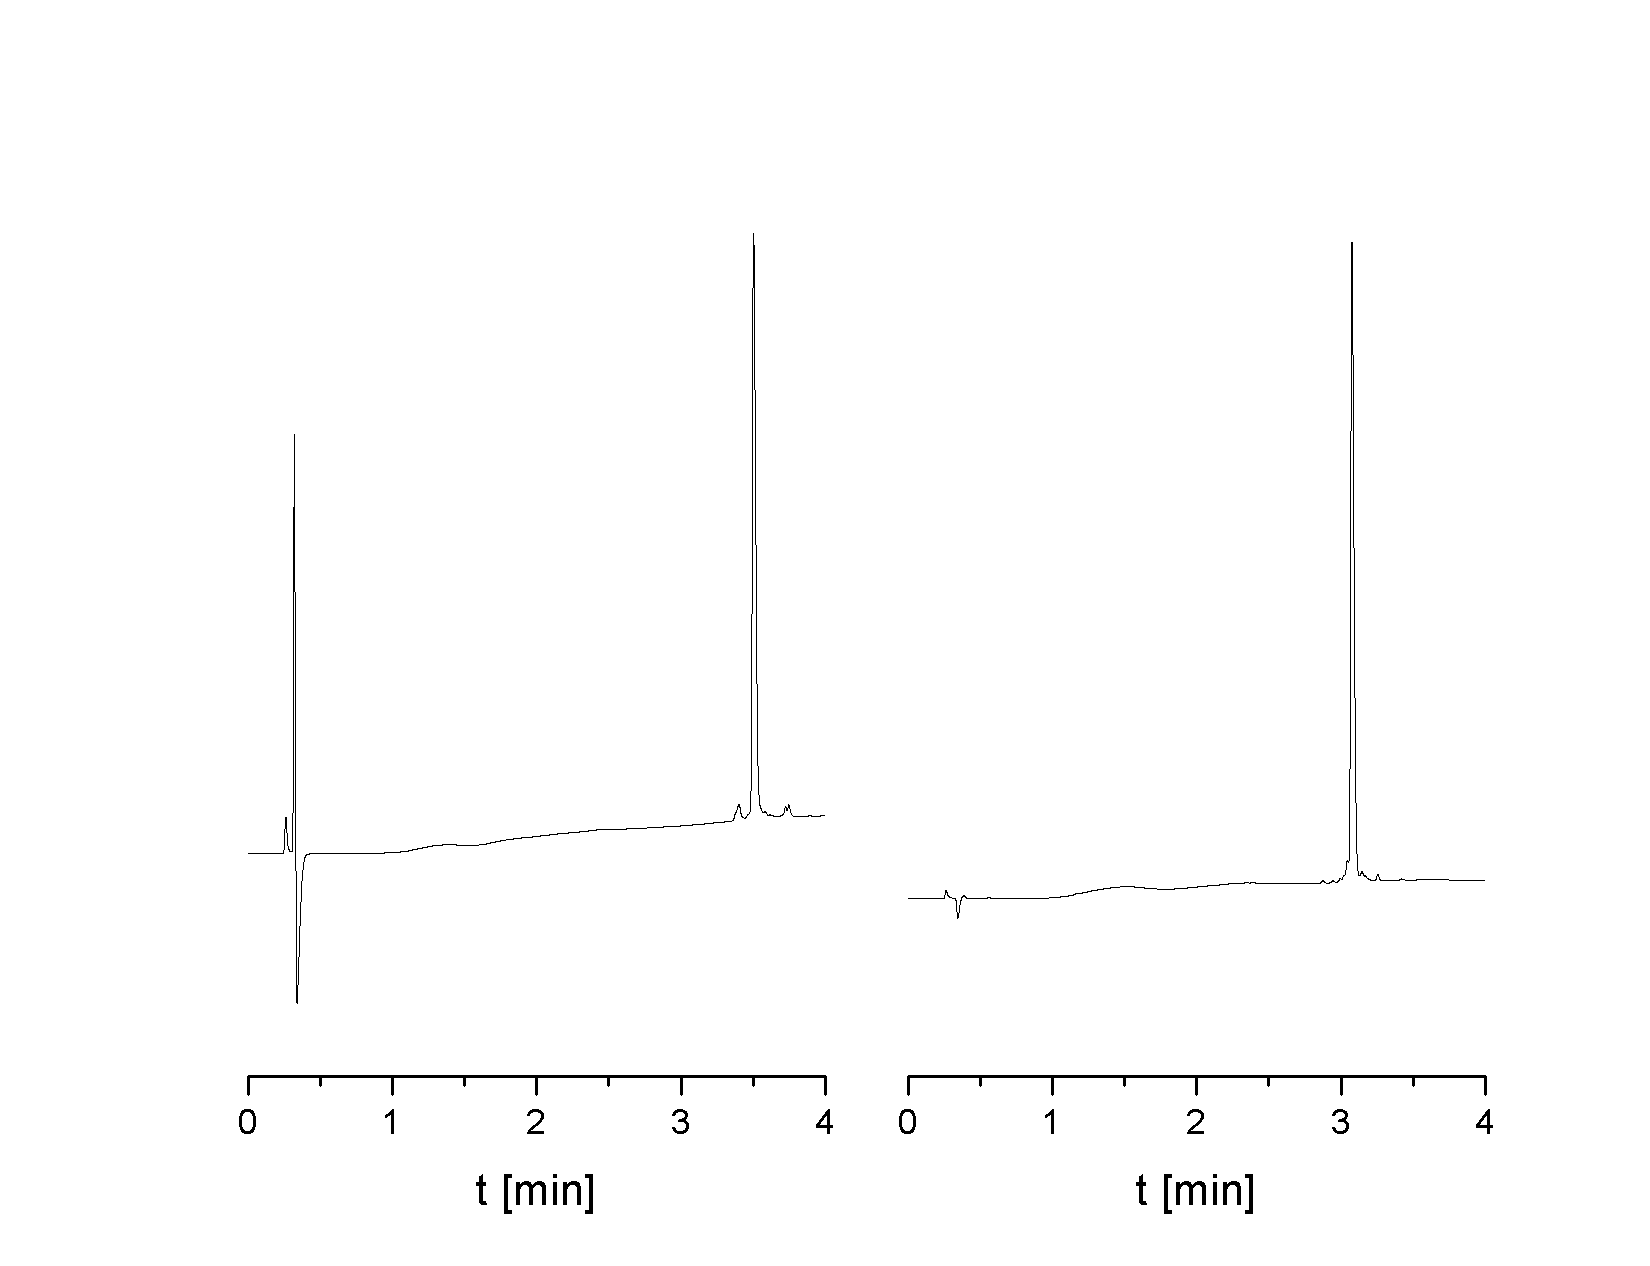
\includegraphics[width=\textwidth]{MeoBrAuxPeps.png}
      \caption{UPLC trace of 4-bromophenyl (\cmpd+{cmpd:auxiliarypeptide.one}) and 4-methoxyphenyl (\cmpd+{cmpd:auxiliarypeptide.two}) auxiliary peptides}
      \label{fig:auxpepuplc}
  \end{figure}

\begin{figure}
    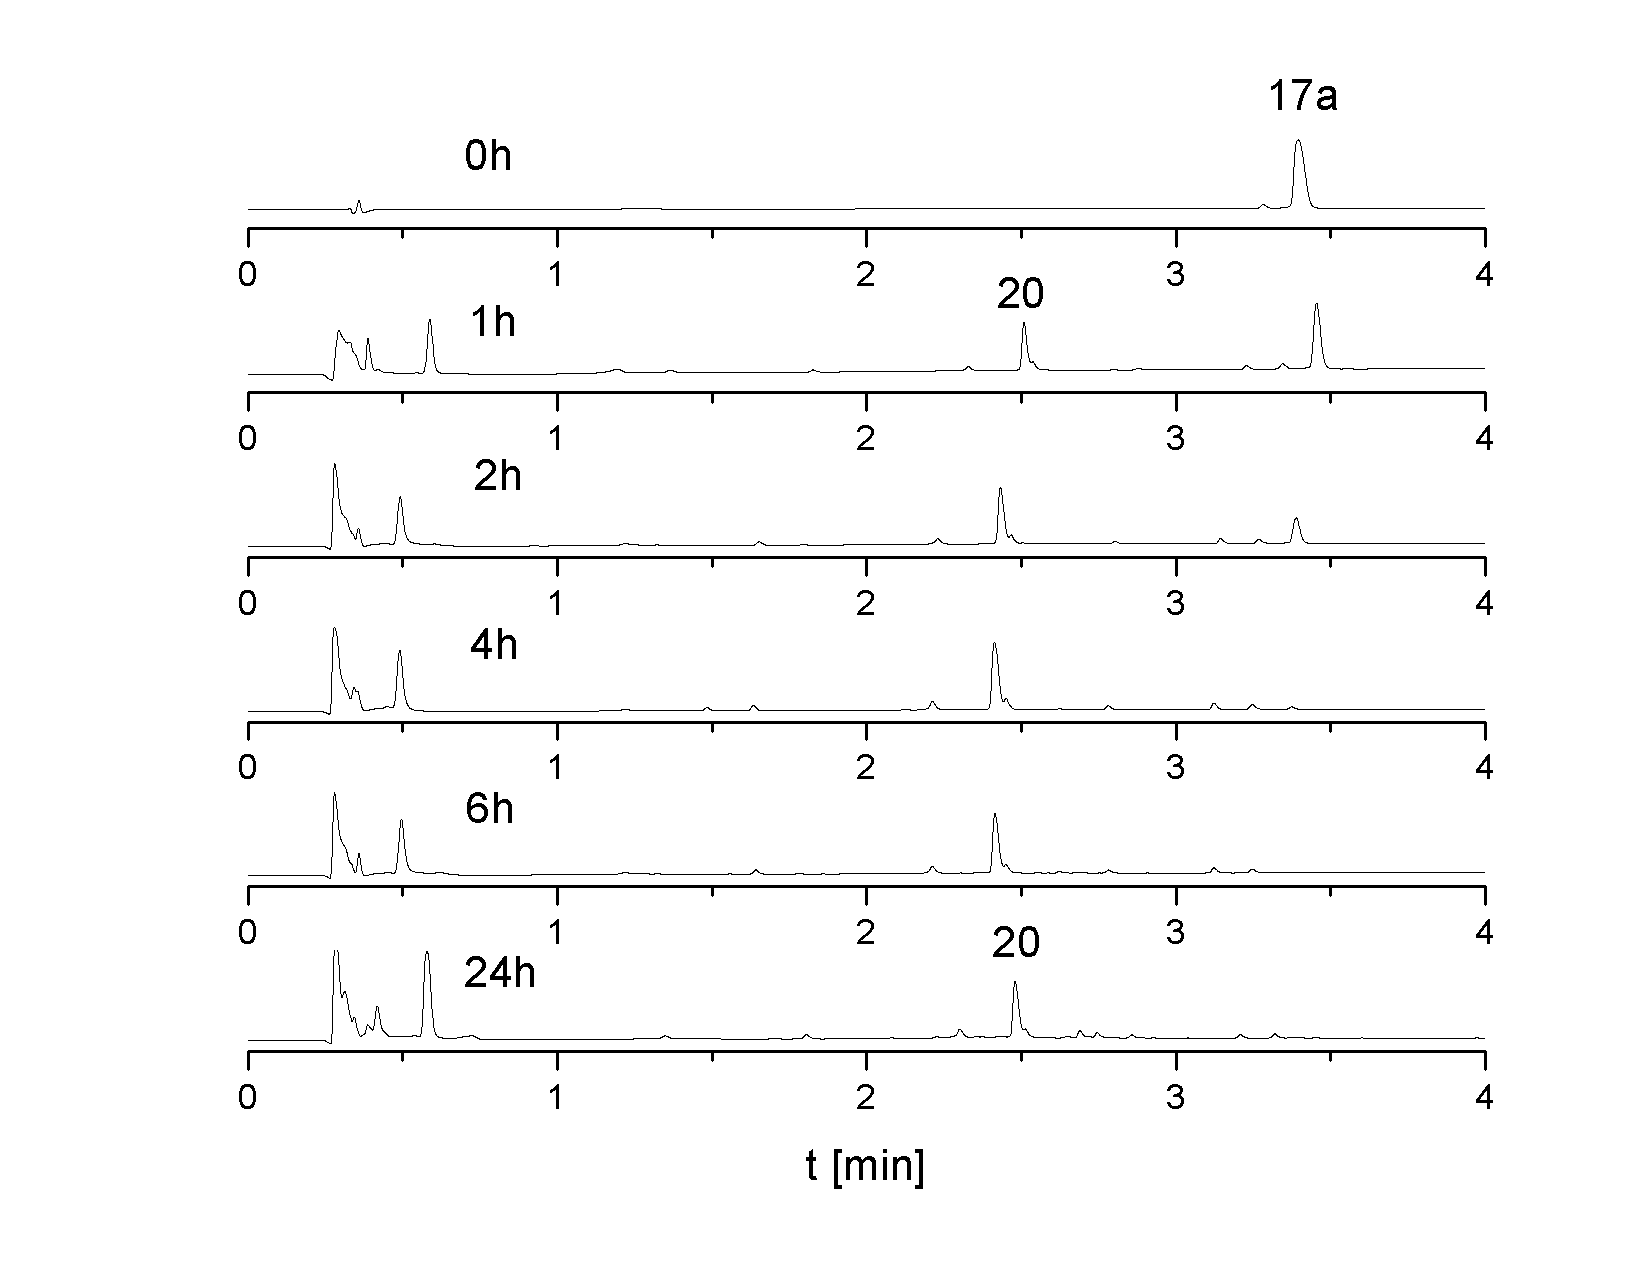
\includegraphics[max width=\linewidth]{br50cleavage.png}
    \caption{UPLC trace for the cleavage of \cmpd+{cmpd:auxiliarydipeptide.one} (100 mM TCEP, \SI{50}{\celsius})}
    \label{fig:br50cleave100}
\end{figure}

\begin{figure}
    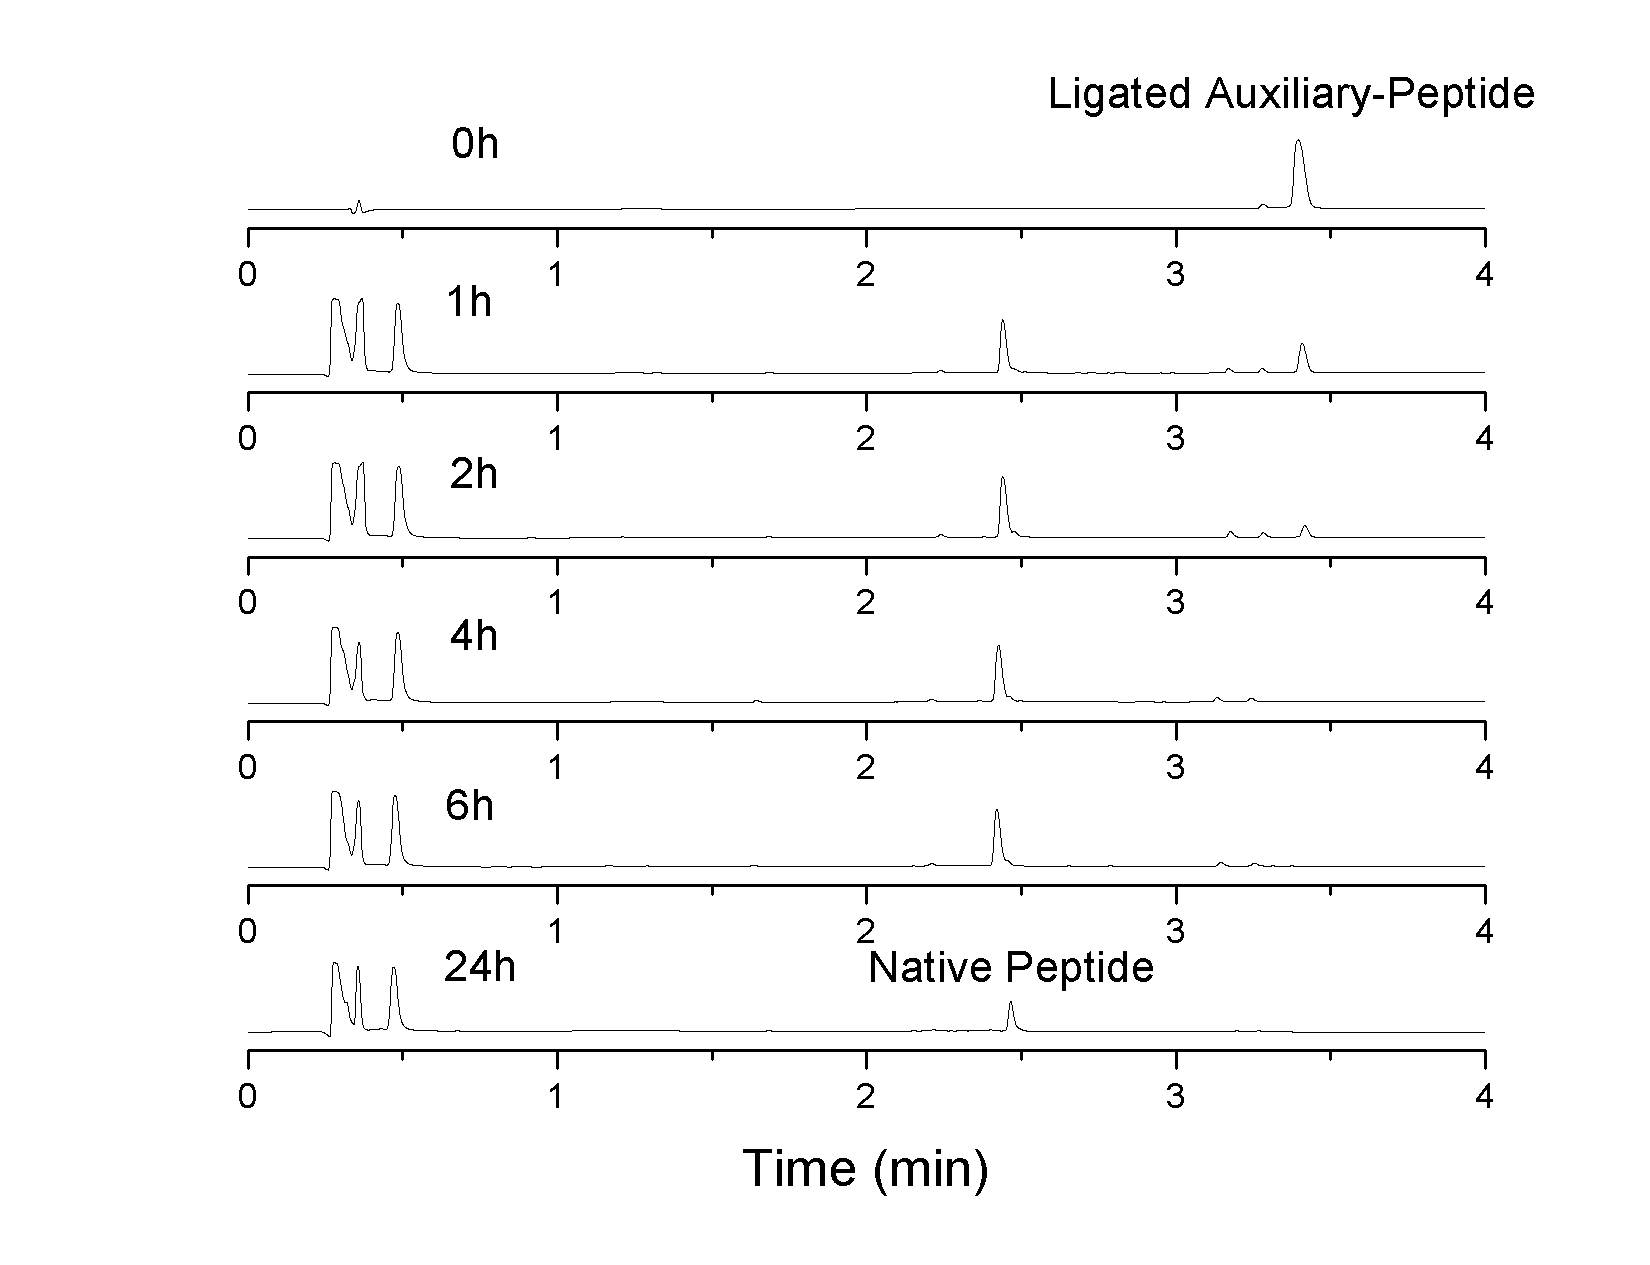
\includegraphics[max width=\linewidth]{brrtcleavage.png}
    \caption{UPLC trace for the cleavage of \cmpd+{cmpd:auxiliarydipeptide.one} (400 mM TCEP, R.T.)}
    \label{fig:brrtcleavage}
\end{figure}

\begin{figure}
    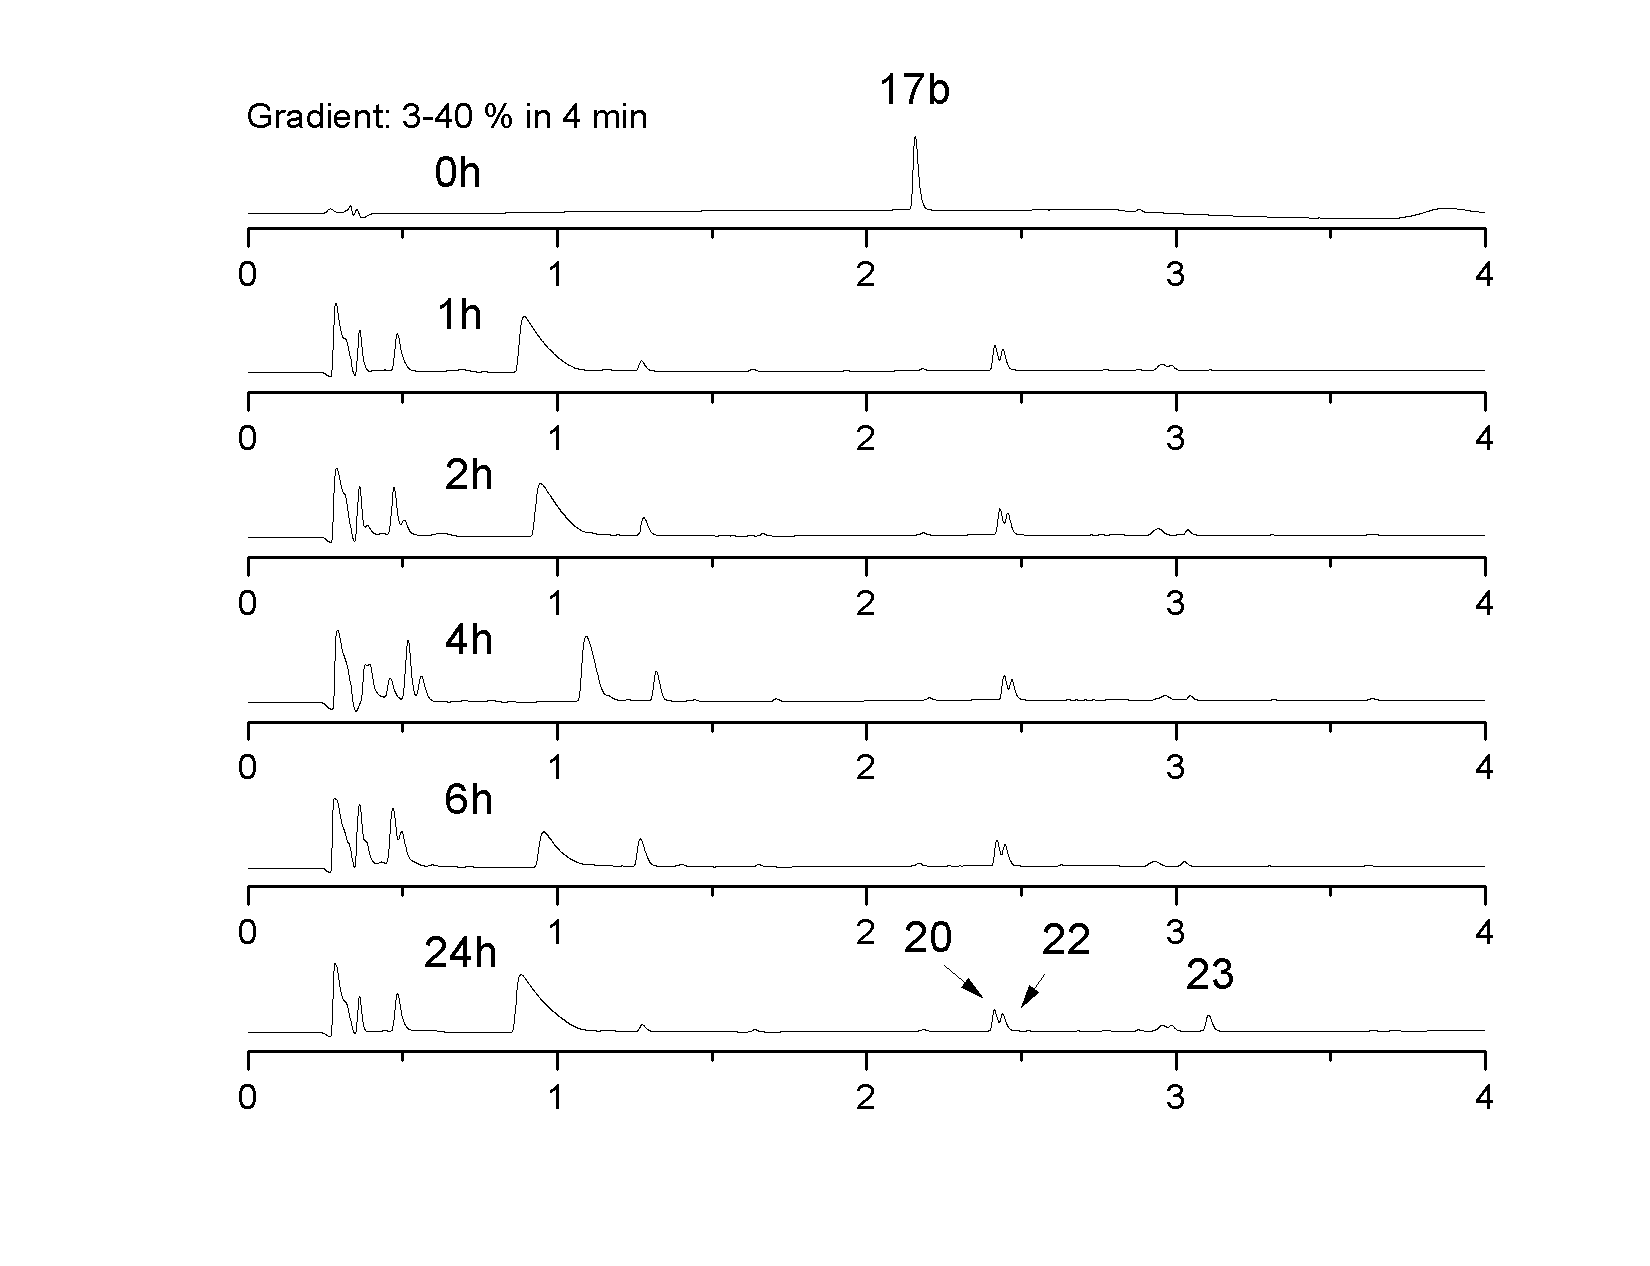
\includegraphics[max width=\linewidth]{meoinitiatorcleavage.png}
    \caption{Side product formation during cleavage of \cmpd+{cmpd:auxiliarydipeptide.two} in the presence of a radical initator (VA-044 20 eq.)}
    \label{fig:meoinitatorcleavage}
\end{figure}

\begin{figure}
    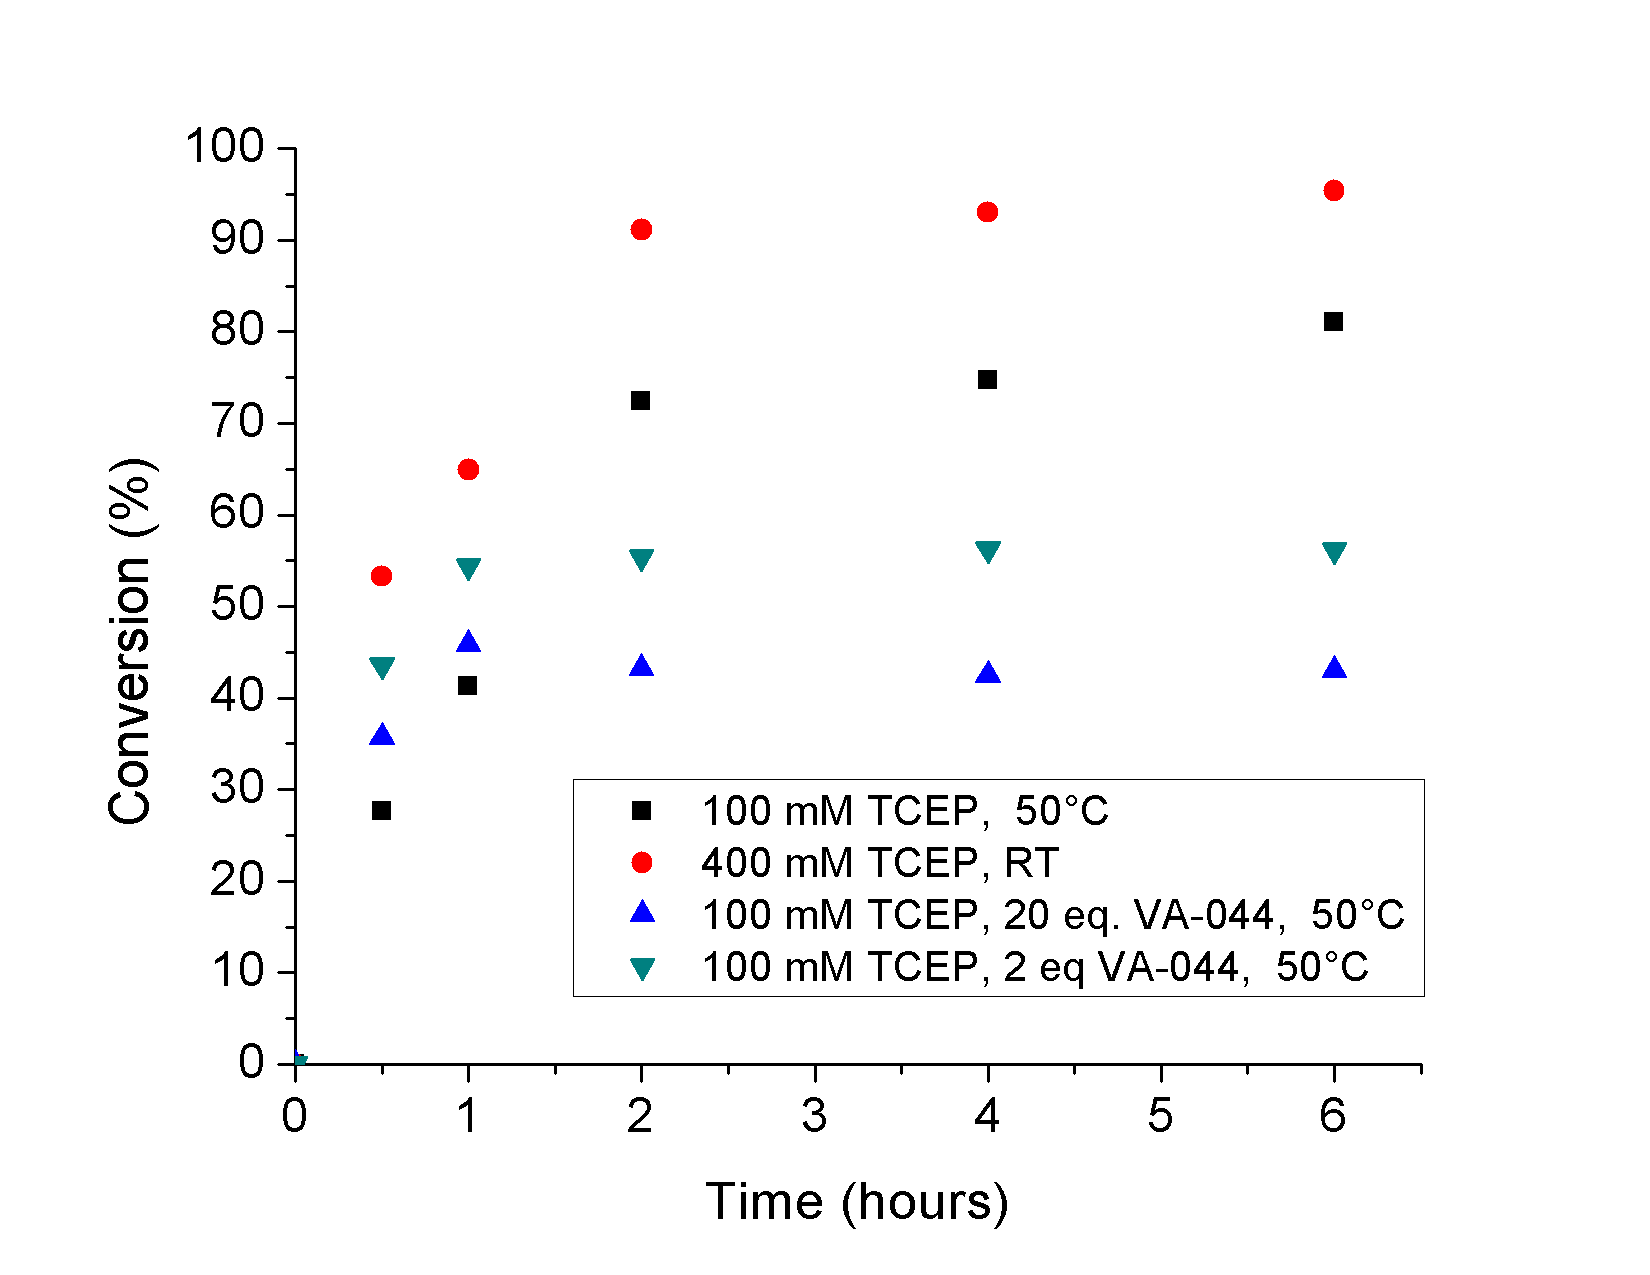
\includegraphics[max width=\linewidth]{meocleavage.png}
    \caption{Rate of auxiliary peptide \cmpd+{cmpd:auxiliarydipeptide.two} cleavage}
    \label{fig:meocleavagerate}
\end{figure}
% ------------------------------------------------------------------------

%%% Local Variables:
%%% mode: latex
%%% TeX-master: "../thesis"
%%% End:


\bibliographystyle{plainnat}
%\bibliographystyle{Classes/CUEDbiblio}
%\bibliographystyle{Classes/jmb}
%\bibliographystyle{Classes/jmb} % bibliography style
\renewcommand{\bibname}{References} % changes default name Bibliography to References
\bibliography{References/references} % References file

\end{document}
